\documentclass{beamer}
\usepackage{tikz}
\usepackage{amsmath}
\usepackage{amssymb}
\usepackage{graphicx}
\usepackage{caption}
\usepackage{cleveref}
\usetheme{Warsaw}
\begin{document}
\title {Gossip vs Markov Chains paper review}
\institute {Ecole Polytechnique fédérale de Lausanne}
\author{Ismail Bouanani and Jean-Baptiste Cordonnier}
\date{May,24th 2016}
\section {Proof outline}




	\begin{frame}
	\begin{itemize}

    \frametitle{ Approximation via Random walks}
    
    \item The problem of rumor spreading is comparable with multiple parrallel     random walks.
   \item  	If node u informs  v, a random walk goes from $u$ to $v$ ( $S_i$=non-lazy), another one remains at $u(S_i=lazy)$. 
   \begin{figure}[h]
\centering
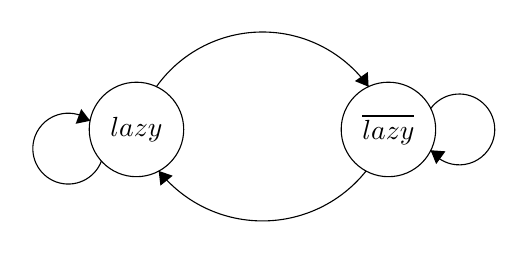
\begin{tikzpicture}[scale=0.2]
\tikzstyle{every node}+=[inner sep=0pt]
\draw [black] (26.1,-26.6) circle (3);
\draw (26.1,-26.6) node {$lazy$};
\draw [black] (42.1,-26.6) circle (3);
\draw (42.1,-26.6) node {$\overline{lazy}$};
\draw [black] (40.688,-29.229) arc (-38.4609:-141.5391:8.413);
\fill [black] (27.51,-29.23) -- (27.62,-30.17) -- (28.4,-29.54);
\draw [black] (27.358,-23.895) arc (144.65362:35.34638:8.265);
\fill [black] (40.84,-23.89) -- (40.79,-22.95) -- (39.97,-23.53);
\draw [black] (23.878,-28.598) arc (-20.31276:-308.31276:2.25);
\fill [black] (23.16,-26.05) -- (22.59,-25.3) -- (22.24,-26.24);
\draw [black] (44.78,-25.277) arc (144:-144:2.25);
\fill [black] (44.78,-27.92) -- (45.13,-28.8) -- (45.72,-27.99);
\end{tikzpicture}

\label{fig:lazyFSM}
\end{figure}

\end{itemize}

	\end{frame}
\begin{frame}
\begin{itemize}
\frametitle{Forward and reversed random walks}
\item Rumor sharing is dual : if $u$ pushes to $v$, $v$ pulls from $u$
\item 2 types of random walks: forward (pushing from a source) and reversed(pulling from a target). 
\item If a forward random walk takes a step from $u$ to $v$, a reversed one   takes a step form $v$ to $u$, if$u$ is the only node pushing to $v$.
\item Reversed random walks are only an analytic tool (no pulls in practice)
 
\end {itemize}

\end{frame}


\begin{frame}
\begin {itemize}
\frametitle{Probabilistic computations}
\item Node $w$ is reached by the information within $k$ rounds if there is k-steps forward (from source) and reversed walk(from $w$) that meet at a certain node.
\item  Union bound over all the possible pairs of patterns of $\{ lazy,non-lazy \}^k$ and all the nodes (we set $k$=T/2).
\begin{align*}
  \scriptsize
  P(w \text{ informed in $T$ rounds}) \geq P(\sum_{S,S'\in \mathcal C_{T/2}, u\in V[G]} X_{s,u}^S Y_{w,u}^{S'} > 0)
\end{align*}
 where $X_{s,u}^S$ and $Y_{w,u}^{S'}$ are indicator random variables on the existence of such walks

\end{itemize}


\end{frame}

\begin {frame}
\begin{itemize}
\frametitle{Matrix coupling (1/2)}
\item We analyze random walks pair wisely. This is done thanks to Markov Chains coupling.
\item Let \textbf{M} and \textbf{M'} two Markov chains, \textbf{M''} represents the joint evolution of both the processes.
\item Here, we use lazy coupling $\mathcal L_{\gamma, \gamma'}(\mathbf{M''})$ which is the coupling of $\mathcal L_\gamma(\mathbf{M})$ with $\mathcal L_{\gamma'}(\mathbf{M'})$ 
  where \[
  \mathcal L _ \gamma (\mathbf{M}) \triangleq (1-\gamma) \mathbf{I} + \gamma \mathbf{M}
\] is the lazy version of \textbf{M} (we add the eventuality of self-edges that occur at a lazy state)

\end{itemize}
\end {frame}


\begin{frame}
\begin{itemize}
\frametitle{Matrix coupling (2/2)}
\item Here, we have to couple different versions of the same Random walk.
\item Doeblin coupling  : 
\[
  \mathcal Q(\mathbf{M})_{(u,w)(v,x)} \triangleq \left\{
    \begin{array}{ll}
      (\mathbf{M} \otimes \mathbf{M})_{(u,w)(v,x)} & u \not = v,\\
      \mathbf{M}_{(u,v)} \cdot \mathbf{1}_{v = x} & u = v.\\
    \end{array}
  \right.
\]
\item Idea of Doeblin coupling : Once two walks meet at the same node $u$, they are never separated again. 

\end{itemize}


\end {frame}

\begin {frame}
\begin{itemize}


 \item We want the stationary distribution of the Doeblin coupling (on the lazy walk) to be as close as possible of the uniform distribution \pi \otimes \pi

\item We have \[
  \norm{u(\mathcal L_{\gamma,\gamma} \circ \mathcal Q(M))^k - \pi \otimes \pi}_2 \leq (1 - \gamma \alpha / 2)^k + 2 \sqrt 2 \gamma \alpha^{-1} n^{-3/2}
\] with $u$ being a distribution over V[G] x V[G] and $\gamma = \min(1/3, \Delta^{0.5-c}\alpha/9)$





\end{itemize}
\end {frame}

\end{document}


